\documentclass{article}

% Code syntax highlighting
% https://www.overleaf.com/learn/latex/Code_Highlighting_with_minted
\usepackage{minted}
\usemintedstyle{borland}

% If you're new to LaTeX, here's some short tutorials:
% https://www.overleaf.com/learn/latex/Learn_LaTeX_in_30_minutes
% https://en.wikibooks.org/wiki/LaTeX/Basics

% Formatting
\usepackage[utf8]{inputenc}
\usepackage[a4paper, margin=1in]{geometry}
\usepackage[titletoc,title]{appendix}
\usepackage{indentfirst}

% Math
% https://www.overleaf.com/learn/latex/Mathematical_expressions
% https://en.wikibooks.org/wiki/LaTeX/Mathematics
\usepackage{amsmath,amsfonts,amssymb,mathtools}
\DeclareMathOperator*{\argmax}{argmax} % thin space, limits underneath in displays


% Images
% https://www.overleaf.com/learn/latex/Inserting_Images
% https://en.wikibooks.org/wiki/LaTeX/Floats,_Figures_and_Captions
\usepackage{graphicx,float}
%Path relative to the main .tex file 
\graphicspath{ {./images/} }

% Tables
% https://www.overleaf.com/learn/latex/Tables
% https://en.wikibooks.org/wiki/LaTeX/Tables

% Algorithms
% https://www.overleaf.com/learn/latex/algorithms
% https://en.wikibooks.org/wiki/LaTeX/Algorithms
\usepackage[ruled,vlined]{algorithm2e}
\usepackage{algorithmic}


% Sections in a new page
% \usepackage{titlesec}
% \newcommand{\sectionbreak}{\clearpage}
% \newcommand{\subsectionbreak}{\clearpage}

\usepackage{hyperref}

\usepackage{multicol}
\usepackage{color}
\setlength{\columnseprule}{1pt}
\usepackage{blindtext}

\begin{document}
\begin{multicols*}{2}

    \section{Chapter 1}
    The \textbf{union} of two events $C = A \cup B$ is the event $C$ where either $A$ occurs or $B$ occurs or both occur

    The \textbf{intersection} of two events $C = A \cap B$ is the event $C$ where both $A$ and $B$ occurs

    The \textbf{complement} of an events $A$ is $A^c$ is the event that A does not occur

    \textbf{Commutative Laws}:
    \begin{itemize}
        \item $A \cup B = B \cup A$
        \item $A \cap B = B \cap A$
    \end{itemize}

    \textbf{Associative Laws}:
    \begin{itemize}
        \item $\left(A \cup B \right) \cup C = A \cup \left( B \cup C \right)$
        \item $\left(A \cap B \right) \cap C = A \cap \left( B \cap C \right)$
    \end{itemize}

    \textbf{Distributive Laws}:
    \begin{itemize}
        \item $\left(A \cup B \right) \cap C = \left( A \cap C \right) \cup \left( B \cap C\right)$
        \item $\left(A \cap B \right) \cup C = \left( A \cup C \right) \cap \left( B \cup C\right)$
    \end{itemize}

    \textbf{Propability measures}
    For mutually disjoint events $A_1, A_2, \dots, A_n$

    $P \left( \cup^\infty_{i=1} A_i \right) = \Sigma^\infty_{i=1}P\left( A_i \right)$

    \begin{center}
        \begin{tabular}{ l p{5cm}}
            Property A & $P\left( A ^ c \right) = 1 - P \left( A \right)$                                                               \\
            Property B & $P \left( \emptyset \right) = 0$                                                                               \\
            Property C & If $ A \subset B$ Then $P \left( A \right) \leq P \left( B \right)$                                            \\
            Property D & $P \left( A \cup B\right) = P \left( A \right) + P \left( B \right) - P \left( A \cap B \right)$, addition law \\
        \end{tabular}
    \end{center}

    $\begin{pmatrix}
            n \\
            r
        \end{pmatrix} = \frac{n!}{\left(n-r\right)! r!}$

    \textbf{Proposition C}: The number of ways that $n$ objects can be grouped into $r$ calsses with $n_i$ in the $i$th class,
    $i=1, \dots, r$ and $\Sigma^r_{i=1}n_i = n$ is
    $\begin{pmatrix}
            n \\
            n_1 n_2 \dots n_r
        \end{pmatrix} = \frac{n!}{n_1! n_2! \dots n_r!}$. This can be extented to multinomial coefficients.
    $\left(x_1 + x_2 + \dots x_r\right) ^ n = \Sigma \begin{pmatrix}
            n \\
            n_1 n_2 \dots n_r
        \end{pmatrix} x_1^{n_1}x_2^{n_2}\dots x_r^{n_r}$

    \textbf{Condiitonal Probability}: Let $A$ and $B$ be two events with $P\left( B \right) \neq 0$.
    The conditional probability of $A$ given $B$ is defined to be $P \left( A \mid B \right) = \frac{P \left( A \cap B \right)}{P \left( B \right)}$

    \textbf{Multiplication Law}: Let $A$ and $B$ be events and assume $P\left( B \right) \neq 0$ Then $P \left( A \cap B \right) = P \left( A \mid B \right) P \left( B \right)$

    \textbf{Law of Total Probability}\\
    Let $B_1, B_2, \dots, B_n$ be such that $\cup^n_{i=1}B_i = \Omega$
    and $B_i \cap B_j = \emptyset$ for $i \neq j$ all with non zero probablity.
    Then for any event $A$: $P \left( A \right) = \Sigma^n_{i=1} P\left( A \mid B_i\right) P \left( B_i\right)$

    \textbf{Bayes Rule}: Let $A$ and $B_1, \dots, B_n$ where the events $B_i$ are disjoint, and non-zero. Then
    $P\left(B_j \mid A \right) = \frac{P \left( A \mid B_j \right) P\left( B_j \right)}{\Sigma^n_{i=1}P \left( A \mid B_i\right) P \left(B_i\right)}$

    \textbf{Independence}. If two events are independent then: $P\left( A \right) = P \left( A \mid B \right) = \frac{P \left( A \cap B\right)}{P \left( B \right)}$ then $P\left( A \cap B \right) = P \left( A \right) P \left( B \right)$

    \section{Chapter 2}
    \textbf{Discrete Random Variable} is a random variable that can take only a finite or at most a countably finite number of values.

    There is a function $p$ such that $P \left( x_i \right) = P \left( X = x_i \right)$ and $\Sigma_i p\left(x_i \right) =1$.
    This function is called the probability mass function or the frequency function of the random variable $X$.

    \textbf{Cumulative Distribution Function} of a random variable $F \left( x \right) = P \left( X \leq x\right)$, $- \infty < x < \infty$.
    The function is non decreasing  $\lim_{x\rightarrow -\infty} F\left( x \right) = 0$ and $\lim_{x\rightarrow \infty} F\left( x \right) = 1$

    \textbf{Bernouli Random Variable}: takes 2 values either 0 or 1 with probabilities $1-p$ and $p$ respectively.

    \[
        \begin{matrix}
            P\left( 1 \right) = p & a                        \\
            P\left( 1 \right) = p & a                        \\
            P\left( 1 \right) = p & if x \neq 0 and x \neq 1
        \end{matrix}
    \]
    \[
        p(x) =\begin{dcases}
            p^x (1-p)^{1-x}, & \text{if} x = 0 \text{ or } x=1 \\
            0,               & \text{otherwise}                \\
        \end{dcases}
    \]
    $E(X) = p$ and $var(X) = p(1-p)$

    \textbf{Indicator Random Vairable} $I_A$ takes the value 1 if $A$ occures and 0 otherwise.
    $I_A$ is a Bernouilli random variable.
    \[
        I_A(\omega) =\begin{dcases}
            1, & \text{if } \omega\in A \\
            0, & \text{otherwise}       \\
        \end{dcases}
    \]

    \textbf{Binomial Distribution}: $n$ experimets, $k$ successes with probability $p$,
    \[
        p(k) = \begin{pmatrix}
            n \\
            k
        \end{pmatrix} p^k \left(1-p\right)^{n-k}
    \]
    $E(X) = np$ and $var(X) = np(1-p)$

    \textbf{Geometric distribution}: with successes probability $p$, probability first success at attempt $X$. $X=k$, so we have $k-1$ failures.
    For $k=1, 2, \dots$
    \[
        p\left( k \right) = P\left( X=k \right) = \left( 1 - p \right)^{k-1}p
    \]

    $E(X) = \frac{1}{p}$ and $var(X) = \frac{1-p}{p^2}$

    \textbf{Negative Geometric distribution}: with successes probability $p$, let $X$ denote total trials. how many tries to get $r$ successes.
    \[
        p(X=k) = \begin{pmatrix}
            k-1 \\
            r-1
        \end{pmatrix} p^r \left( 1-p \right)^{k-r}
    \]
    $E(X) = \frac{k}{p}$ and $var(X) = \frac{(1-p)k}{p^2}$

    \textbf{Hypergeometric distribution}: If a bag has $n$ balls, of which $r$ are black and $n-r$ are white.
    Let $X$ denote the number of black balls drawn then taking $m$ balls without replacement
    \[
        p(X=k) =\frac{ \begin{pmatrix}
                r \\
                k
            \end{pmatrix} \begin{pmatrix}
                n-r \\
                m-k
            \end{pmatrix}}{ \begin{pmatrix}
                n \\
                m
            \end{pmatrix}}
    \]
    $E(X) = \frac{mr}{n}$ and $var(X) = \frac{mr(n-r)(n-m)}{n^2(n-1)}$

    \textbf{Poisson frequency function}: with parameter $\lambda, \lambda > 0$
    \[
        p(X=k) = \frac{\lambda^k}{k!}e^{-\lambda}
    \]
    $e^\lambda = \Sigma^\infty_{k=0} \left(\frac{\lambda^k}{k!}\right)$

    The \textbf{Poisson distribution} can be derived as the limit of a binomial distribution as the number of trials $n$ approached infinity.
    and the probability of success on each trial $p$ approaches zero such that $np=\lambda$
    \[
        p(k) = \frac{n!}{k! (n-k)!} p^k (1-p)^{n-k}
    \]
    $E(X) = \lambda$ and $var(X) = \lambda$

    \textbf{Continuous Random Variable}: can take on a continuum of values, not a set value.
    The probability $X$ lies between $a$ and $b$ is the areas under the curve.
    $P(a < X < b) = \int^b_a f(x)dx$, and  $\int^\infty_{-\infty} f(x)dx = 1$.
    $P(a < X < b) = P(a \leq X < b)  = P(a < X \leq b) $

    For small $\delta$ if $f$ is continuous at $x$, $P(x-\frac{\delta}{2} \leq X \leq x+\frac{\delta}{2}) = \int^{x+\frac{\delta}{2}}_{x-\frac{\delta}{2}}f(u)du \approx \delta f(x)$

    The \textbf{cumulative distribution function} of a continuous random variable is $F(x) = P(X \leq x)$, where $F(x) = \int^x_{-\infty}f(u)du$.
    From calculus $f(x) = F^\prime(x)$

    \textbf{Uniform distribution}, To pick value over inter $\left[a, b\right]$, denoted $X~U(a, b)$. the pdf:
    \[
        f(x) =\begin{dcases}
            \frac{1}{b-a}, & \text{for } a \leq x \leq b \\
            0,             & \text{otherwise}            \\
        \end{dcases}
    \]
    $E(X) = \frac{a+b}{2}$ and $var(x) = \frac{(b-a)^2}{12}$

    The cumulative distribution function of uniform distribition:
    $F_X(x) = \int_{-\infty}^xf_X(y)dy = \begin{dcases}
            0,               & \text{if } x < a            \\
            \frac{x-a}{b-a}, & \text{for } a \leq x \leq b \\
            1,               & \text{if } x \geq b         \\
        \end{dcases}$

    \textbf{The Exponential Density}
    \[
        f(x) =\begin{dcases}
            \lambda e^{-\lambda x}, & x \geq 0 \\
            0,                      & x < 0    \\
        \end{dcases}
    \]
    $E(X) = \frac{1}{\lambda}$ and $var(x) = \frac{1}{\lambda^2}$

    The cumulative distribution function of exponential distribution:
    $F_X(x) = \int_{-\infty}^xf_X(y)dy = \begin{dcases}
            \lambda e^{-\lambda x} & \text{for } x > 0    \\
            0,                     & \text{for } x \leq 0 \\
        \end{dcases}$

    \textbf{Memoryless Property}: The exponential distribution satisfy the following property: $P(X > s+t | X>s) = P(X > t)$

    \textbf{The Gamma Density Function}: depending on $\alpha$, shape patameter, and $\lambda$, scale parameter. If $t < 0, g(t) = 0$
    \[
        g(t) = \frac{\lambda^a}{\Gamma(\alpha)}e^{\alpha-1}r^{-\lambda t}, t \geq 0
    \]
    \[
        \Gamma(x) = \int^\infty_0 u^{x-1}e^{-u} du, x > 0
    \]
    By integration by parts $\Gamma(a) = (a-1)\Gamma(a-1)$

    $E(X)=\frac{\alpha}{\lambda}$ and $Var(x) = \frac{\alpha}{\lambda^2}$

    \textbf{Normal Distribution}: based on Central limit theorem.
    Depending on $\mu$, mean, and $\sigma$, the standard deviation. $X~N\left(\mu, \sigma^2\right)$
    $f(x) = \frac{1}{\sigma\sqrt{2\pi}}e^{e(x-\mu)^2/2\sigma^2}$


    If $Z~N(0, 1)$
    The probability density function $\phi(x) =\frac{1}{\sqrt{2\pi}} e^{-X^2/2}$
    The cumulatif density function $\Phi(x) =\frac{1}{\sqrt{2\pi}} \int_{-\infty}^x e^{-y^2/2}dy$

    $E(X) = \mu$ and $var(x) = \sigma^2$

    \textbf{Beta Density}: The beda density is useful for modeling ranodm variables that are restricted to the interval $\left[0, 1\right]$:
    $f(u) = \frac{\Gamma(a+b)}{\Gamma(a) \Gamma(b)} u^{a-1} (1-u)^{b-1}, 0 \leq u \leq 1$

    \textbf{Functions as random Variables}

    \textbf{Proposition A}: If $X~N(\mu, \sigma^2)$ and $Y=aX+b$, then $Y~N(a\mu +b, a^2\sigma^2)$

    \textbf{Proposition B}: Lex $X$ be a continuous random variable with density $f(x)$ and let $Y=g(x)$
    where $g$ is differentiable, strictly monotonic function on some intertal $I$.
    Suppose that $f(x) = 0$ if $x$ is not in $I$.
    Then $Y$ has the density function $f_Y(y) = f_X(g^{-1}(y))) \left| \frac{d}{dy}g^{-1}(y) \right|$.
    For $y$ such that $y=g(x)$, for some $x$, and $f_Y(y) = 0$ if $y \neq g(x)$ for any $x$ in $I$.

    \textbf{Proposition C}:
    Let $Z=F(X)$; then $Z$ has a uniform distribution on $\left[0, 1\right]$

    \textbf{Proposition D}:
    Let $U$ be uniform on $\left[0, 1\right]$, and let $X=F^{-1}\left(U\right)$. Then the cdf of $X$ is $F$.

    \section{Chapter 3}

    The joint behavior of two random variables $X$ and $Y$, is determined by the cumulative distribution function $F(X, y) = P(X \leq x, Y \leq y)$.
    Regardleess of whether $X$ and $X$ are continuous or discrete.
    This can be extented to $P(x_1 < X \leq x_2, y_1 < Y \leq y_2) = F(x_2, y_2) - F(x_2, y_1) - F(x_1, y_2) + F(x_1, y_1)$

    \textbf{Discrete Random Variables}.
    Suppose that $X$ and $Y$ are discrete random variables defined on the same sample space.
    Their \textbf{joint frequency function}, or joint probability mass function $p(x, y)$ is $p(x_i, y_j) = P(X=x_i, Y=y_j)$

    To find the frequency function of $Y$, we simply sum down the appropiate column of the table.
    For this reason $P_Y$ is called the marginal frequency funciton of $Y$.
    $P_X(x) = \Sigma_i p(x, y_i)$ is the marginal frequency function of $X$.

    \textbf{Continuous Random Variables}:
    Suppose that $X$ and $Y$ are continuous random variables with a joing cdf, $F(x, y)$.
    Their \textbf{joint density function} is a pievewise continous funciton of two variables $f(x, y)$.
    The density funciton $f(x, y)$ is nonnegative and $\int^\infty_{\infty} \int^\infty_{\infty} f(x, y) dy dx = 1$

    For 2 dimentional set of $A$: $P((X, Y) \in A) = \int \int_A f(x, y) dy dx$.
    In particular, if $A = \left\{ (X, Y) \vert X\leq x \text{ and } Y \leq y \right\}$
    $F(x, y) = \int_{-\infty}^x \int_{-\infty}^y f(u, v) du dv$.
    To generalize $f(x, y) = \frac{\partial^2}{\partial x \partial y} F(x, y)$

    for small $\delta_x$ and $\delta_y$, if $f$ is a continuous at $\left( x, y \right)$:
    $P( x \leq X \leq x + \delta_x , y \leq Y \leq y + \delta_y) = \int_x^{x+\delta_x} \int_y^{y+\delta_y} f(u, v) dv du \approx f(x, y) \delta_x \delta_y$

    The marginal cdf of $X$ or $F_X$, is $F_X(x) = P(X \leq x) = \lim_{y\rightarrow \infty}F(x, y) = \int_{-\infty}^x \int_{-\infty}^\infty f(u, y) dy du$.
    From this, it follows tha tthe density function of $X$ alone, known as the marginal density of $X$ is $f_X(x) = F^\prime_X(x) = \int^\infty_{-\infty} f(x, y)dy$
    In the discrete case, the marginal frequency function was found by summing the joint frequency funciton over the other variable, in the continous case it is found by integration.

    In someapplications, it is usefyl to analyze distributions that are uniform over some region of Space. For example, in the plane, the random point $\left(X, Y\right)$ is uniform over a region $R$, if for any $A \subset R$
    $P((X, Y) \in A) = \frac{\left| A \right|}{\left| R \right|}$

    \textbf{Independent Random Variables}: Random Variables $X_1, X_2, \dots X_n$ are said to be independent if therir joint cdf
    factors into the product of their marginal cfds: $F(x_1, x_2, \dots x_n) = F_{X_1}(x_1)F_{X_2}(x_2)\dots F_{X_n}(x_n)$ for all $x_1, x_2, \dots x_n$

    Independence holds for both continuous and discrete random variables.
    $F(x, y) = F_X(x)F_Y(y)$ as well as $P(X\in A, Y \in B) = P(X\in A) P (Y \in B)$

    \textbf{Conditional distrbution}.

    For discrete case: $P(X=x_i | Y=y_j) = \frac{P(X=x_i, Y=y_j)}{P(Y=y_j)} = \frac{P_{XY}(x_i, y_j)}{P_Y(y_j)}$
    Thus consequently $P_{XY}(x, y) = P_{X|Y}(x|y)P_Y(y)$ and $P_X(x) = \Sigma_y P_{X|Y}\left(x|y\right) P_Y(y)$

    For continunous case: $f_{Y|X}(y|x) = \frac{f_{XY}(x, y)}{f_X(x)}$.
    We can then solve $P(y \leq Y \leq y + dy | x \leq X \leq X+dx) = \frac{f_{XY}(x, y)dx dy}{f_X(x) dx} = \frac{f_{XY}(x, y)}{f_X(x)}dy$
    The joint density can be expressed in terms of the marginal and conditional densities:
    $f_{XY}(x, y) = f_{Y|X}(y|x)f_X(x)$, integrating both sides over $x$ allows us to get the marginal density of $Y$ to be expressed as
    $f_Y(y) = \int_{-\infty}^\infty f_{Y|X}(y|x)f_X(x) dx$

    Suppose that $X$ and $Y$ are discrete random variables, and we have $Z = X + Y$. to get the frequency function of $Z$.
    $Z=z, \text{ if } X=x \text{ and } Y =z-x$.
    $P_Z(z) = \Sigma^\infty_{x=-\infty} p(x, z-x)$
    If $X$ and $Y$ are independent, $p(x, y) = P_X(x)P_Y(y)$ and $P_Z(z) = \Sigma^\infty_{x=-\infty}P_X(x)P_Y(z-x)$

    To generalize $F_Z(z) = \int^\infty_{-\infty} \int^z_{-\infty} f(x, u-x) du dx = \int^z_{-\infty} \int^\infty_{-\infty} f(x, u-x) dx du$
    Which we can differentiate to get $f_Z(z) = \int^\infty_{-\infty} f(x, z-x) dx$

    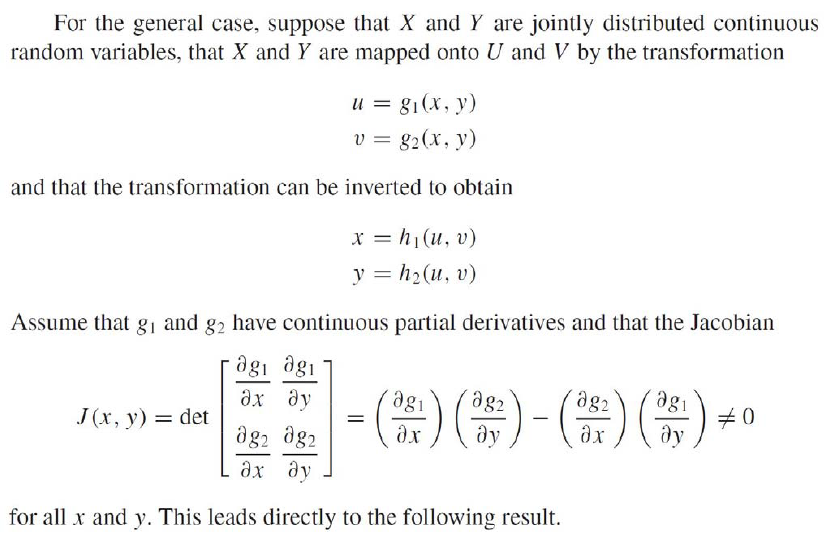
\includegraphics[width=0.9\columnwidth]{3_6_2_1.png}
    \textbf{Proposition A}: Under the assumptions just stated, the joint density of $U$ and $V$ is:
    $f_{UV}(u, v) = \frac{F_{XY}(h_1(u, v), h_2(u, v))}{J(h_1(u, v), h_2(u, v))}$.
    For $(u, v)$ such that $u=g_1(x, y)$ and $v=g_2(x, y)$ for some $(x, y)$ and 0 elsewhere

    \textbf{Extrema and Order Statistics}
    The density of $X_{(k)}$, the $k$th-order statistic, is $f_k(x) = \frac{n!}{(k-1)! (n-k)!}f(x) F^{k-1}(x) \left[1-F(x)\right]^{n-k}$

    \section{Chapter 4}

    \textbf{Expected Value}, also known as mean.
    For discrete random variable $X$ with frequency function $p(x)$, the expected value of $X$, denoted $E(X)$ is $E(X) = \Sigma_i x_i p(x_i)$
    Provided the sum is less than infinity, if the sum diverges, the expectation in undefined.

    For continuous ranodm variable with density $f(x)$, then $E(X) = \int_{-\infty}^\infty xf(x) dx$

    If $X$ is a nonnegative continuous random variable $E(X) = \int^\infty_0 \left[1-F(X)\right] dx$

    \textbf{markov's inequality}: if $X$ is a ranodm variable with $P(X \geq 0) = 1$ and for which $E(X)$ exists, then $P(X \geq t) \leq E(X) / t$

    \textbf{Expectation of Functions of Random Variables}

    \textbf{Thoerem A}
    Suppose that $Y=g(X)$.
    if $X$ is discrete with frequency function $p(x)$ then $E(Y) = \Sigma_xg(x)p(x)$
    if $X$ is continuous with frequency function $f(x)$ then $E(Y) = \int_{-\infty}^\infty g(x)f(x) dx$

    \textbf{Thoerem B}
    Suppose that $X_1, \dots, X_n$ are jointly distributed random variables and $Y=g(X_1, \dots, X_n)$.
    if $X_i$ are discrete with frequency function $p(x_1, \dots, x_n)$ then $E(Y) = \Sigma_{x_1,\dots, x_n} g(x_1, \dots, x_n) p(x_1, \dots, x_n)$
    if $X_i$ are continuous with frequency function $f(x_1, \dots, x_n)$ then $E(Y) = \int \dots \int g(x_1, \dots, x_n) f(x_1, \dots, x_n) dx_1\dots dx_n$

    \textbf{Corollary A}:
    If $X$ and $Y$ are independent random variables and $g$ and $h$ are fixed functions,
    the $E\left[g(X) h(Y)\right] = \left\{E[g(X)]\right\} \left\{ E[h(Y)] \right\}$,
    provided that the expectations on the right-hand side exists

    \textbf{Expectations of Linear Combinations of Random Variables}:

    \textbf{Theorem A}:
    if $X_1, \dots, X_n$ are jointly distributed random variables with $E(X_i)$ and $Y$ is a linear funciton of the $X_i$.
    $Y = a + \Sigma_{i=1}^nb_iX_i$ then $E(Y) = a + \Sigma_{i=1}^nb_i E(X_i)$

    \textbf{Variance}: if $X$ is a random variable with expected value $E(X)$, the variance of $X$ is
    $Var(X) = E \left( \left[ X - E(X) \right]^2 \right)$.
    Provided that the expectation exists. The standard deviation of $X$ is the square root of the variance.

    if $X_i$ are discrete with frequency function $p(x)$ with mean $\mu$ then $Var(Y) = \Sigma_i \left( x_i - \mu \right)^2 p(x_i)$
    if $X_i$ are continuous with frequency function $f(x)$ with mean $\mu$ then $Var(Y) = \int_{-\infty}^\infty \left( x-\mu \right)^2 f(x) dx$

    \textbf{Theorem A}: If $Var(X)$ exists, and $Y=a + bX$, then $Var(Y) = b^2 Var(X)$

    \textbf{Theorem B}: If $Var(X)$ exists, can be calculated ad $Var(X) = E(X^2) - \left[E(X)\right]^2$

    \textbf{Theorem C}: Let $X$ is a random variable with mean $\mu$ and variance $\sigma^2$. Then for any $t>0$:
    $P(|X-\mu| > t) \leq \frac{\sigma^2}{t^2}$

    \textbf{Corollary A}: if $Var(X) = 0$, then $P(X=\mu) = 1$

    \textbf{Error Measurement}: if an expetiment $X$ is modeled as $X = x_0 + \beta + \epsilon$.
    we have $E(X) = x_0 + \beta$ and $Var(X) = \sigma^2$. $x_0$ is real value, $\beta$ is constant error, $\epsilon$ is random error.
    The mean squared error $MSE = E\left[ \left( X - x_0\right)^2 \right]$
    \textbf{Theorem A}: $MSE = \beta^2 + \sigma^2$

    \textbf{Covariance}:
    The covariance of two random variables measure is a measure of the jion probability of 2 or more variables.
    if $X$ and $Y$ are jointly distributed random variables with expectectations $\mu_X$ and $\mu_Y$, respectively.
    The covariance of $X$ and $Y$ is $Cov(X, Y) = E\left[ (X-\mu_X) (Y-\mu_Y) \right] = E(XY) - E(X)E(Y)$.
    If $X$ and $Y$ are independent, then $E(XY) = E(X)E(Y)$ and $Cov(X, Y)=0$

    \textbf{Theorem A}: Suppose that $U = a + \Sigma_{i=1}^n b_i X_i$ and $V = c + \Sigma_{j=1}^m d_j Y_j$
    Then $Cov(U, V) = \Sigma_{i=1}^n \Sigma_{j=1}^m b_i d_j Cov(X_i, Y_j)$

    $Var(X + Y) = Cov(X+Y, X+Y) = Var(X) + Var(Y) + 2Cov(X, Y)$

    \textbf{Corollary A}: $Var(a + \Sigma_{i=1}^n b_i X_i) = \Sigma_{i=1}^n \Sigma_{j=1}^n b_i b_j Cov(X_i, X_j)$

    \textbf{Corollary B}: $Var(\Sigma_{i=1}^n X_i) = \Sigma_{i=1}^n Var(X_i)$, if $X_i$ are independent

    \textbf{Correlation coefficient}: If $X$ and $Y$ are jointly distributed random variables with existingi variances and covariances that are non zero.
    Then the correlation of $X$ and $Y$, denoted $\rho = \frac{Cov(X, Y)}{\sqrt{Var(X) Var(Y)}}$
    $\rho = \frac{\sigma_{XY}}{\sigma_X \sigma_Y}$
    and $\sigma_{XY} = \rho \sigma_X \sigma_Y$

    \textbf{Theorem B}: if $-1 \leq \rho \leq 1$. Furthermore, $\rho = \pm 1$ if and only if $P(Y = a + bX) = 1$ for some constants $a$ and $b$.

    \textbf{Conditional Expectation}:
    Suppose $Y$ and $X$ are discrete random variables and that the conditional frequency function of $Y$ given $x$
    is $p_{Y|X}(y|x)$. The conditional expectation of $Y$ given $X=x$ is $E(Y |X=x) = \Sigma_y y p_{Y|X}(y|x))$
    For the continuous case: $E(Y |X=x) = \int y f_{Y|X}(y|x)) dy$. Or generally
    \[
        E(h(Y) |X=x) = \int h(y) f_{Y|X}(y|x)) dy
    \]

    \textbf{Theorem A}: $E(Y) = E \left[ E(Y|X) \right]$

    \textbf{Theorem B}: $Var(Y) = Var\left[ E(Y|X) \right] + E\left[ Var(Y|X) \right]$

\end{multicols*}


\end{document}
